\newpage
\section{Overview}
\label{chapter1}

%This core provides a APB controller in a VHDL file which can be instantiated into Cobham Gaisler NOEL-V Multiprocessor System.

SafeDE is a flexible Diversity Enforcement hardware module that provides a solution for light-lockstepping execution, an alternative to conventional lockstep. In contrast to the traditional lockstep solution, in the light-lockstep approach, there are two independent cores that can execute either critical tasks in lockstepped execution or non-critical tasks independently. For that purpose, SafeDE is instantiated in the SoC as an APB slave\footnote{Based on AMBA 2.0 specification} and couples two cores, forcing them to keep some staggering \footnote{Difference of executed instructions between two cores executing the same software} and introducing time diversity to avoid common cause faults.

\begin{figure}[H]
	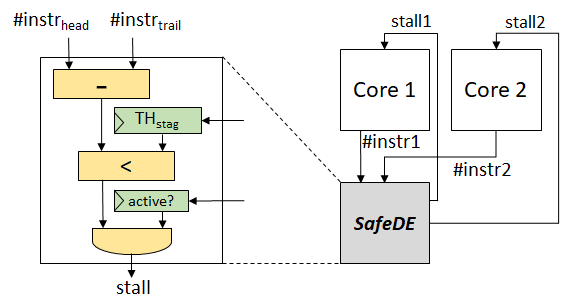
\includegraphics[keepaspectratio,width=\columnwidth]{img/safede}
        \caption{Simplified light-lockstep scheme with SafeDE.}
	\label{fig:simplified_scheme}
\end{figure}
In figure \ref{fig:simplified_scheme} it is shown a simplified light-lockstep scheme with SafeDE. When active, SafeDE counts the instructions executed by both cores. Each cycle, SafeDE computes the staggering substrating those instructions executed by the trail core to the ones executed by the head core. If that difference (staggering) is smaller than a given threshold, the trail core is stalled.

A light-lockstep execution implemented with SafeDE offers some advantages in contrast with the classical lockstep approach:
\begin{itemize}
	\item \textbf{Low-cost:} SafeDE employs few hardware resources.
	\item \textbf{Flexibility:} SafeDE can be enabled and disable at will. This allows the possibility of using a couple of cores to execute either two tasks with SafeDE disabled or one task with SafeDE enabled, depending on its criticality.
        \item \textbf{Low intrusiveness:} SafeDE can be implemented in a SoC performing only a few modifications in the design. Namely, SafeDE needs only the instruction counters and two signals to stall the cores. 
\end{itemize}

When working in light-lockstep mode, both cores have to execute exactly the same instructions so that software does not diverge. For that reason, they need to execute redundant independent processes allocated in different segments of memory. Even though SafeDE guarantees time diversity, a software mechanism to detect the discrepancies in the results of both cores has to be implemented. SafeDE is devised to work in bare metal since an operating system could make the paths of the redundant cores diverge (e.g. interruptions, exceptions).

\hspace{5cm}
